\documentclass[11pt,a4paper]{article}
\usepackage{amsmath,amssymb,amsthm}
\usepackage{geometry}
\geometry{margin=1in}
\usepackage{hyperref}
\usepackage{enumitem}
\usepackage{tikz}
\usetikzlibrary{trees,shapes}
\usepackage{xcolor}

\newtheorem{theorem}{Theorem}[section]
\newtheorem{lemma}[theorem]{Lemma}
\newtheorem{proposition}[theorem]{Proposition}
\newtheorem{corollary}[theorem]{Corollary}
\newtheorem{definition}[theorem]{Definition}
\theoremstyle{remark}
\newtheorem{remark}[theorem]{Remark}

\title{\bfseries A Rigorous Harmonic Sine Transform\\
\large From Greedy Decomposition to Zeta‑Regularised Spectra\\
\large Revised Foundation}
\author{}
\date{}

\begin{document}
\maketitle

\begin{abstract}
Victor Geere's greedy harmonic reconstruction of the sine function uses the fractions \(\pi/(n+2)\) and leads to a complete binary partition of \([0,\pi]\)—the \emph{greedy harmonic tree}. We show that the natural basis formed by the digit functions \(\delta_n\) does \emph{not} yield a Riesz basis; the obstacle is removed by constructing an orthonormal Haar basis adapted to the tree. This basis gives a rigorous Harmonic Sine Transform (HST) that is an isometric isomorphism onto \(\ell^2\). The arithmetic properties of the greedy expansion are encoded faithfully: the threshold angles \(\theta_n^*\), the correlation kernel \(K(n,m)\), and the logarithmic selection density all reappear as inner products of the Haar basis. We then define the HST Dirichlet series, deduce its meromorphic continuation, and formulate a Weil‑type explicit formula linking its values at the non‑trivial zeros of \(\zeta(s)\) to sums over prime powers. Finally, we construct a family of self‑adjoint operators whose Fredholm determinants vanish precisely at the Riemann zeros, providing a new operator‑theoretic realisation of the Hilbert–Pólya idea.
\end{abstract}

\tableofcontents

\section{Introduction: Geere's Greedy Sine Decomposition}

Fix the \emph{harmonic fractions}
\[
\alpha_n = \frac{\pi}{n+2}, \qquad n = 0,1,2,\dots .
\]
For any angle \(\theta\in[0,\pi]\) define recursively
\[
\begin{aligned}
\theta_0 &= 0,\\
\delta_n(\theta) &= \Theta\bigl(\theta - \theta_n - \alpha_n\bigr) \in\{0,1\},\\
\theta_{n+1} &= \theta_n + \delta_n(\theta)\,\alpha_n,
\end{aligned}
\tag{1}
\]
where \(\Theta\) is the Heaviside step function. The sequence \(\bigl(\delta_n(\theta)\bigr)_{n\ge0}\) is the \emph{greedy harmonic digit sequence} of \(\theta\). For a.e.\ \(\theta\) we have the convergent expansion
\[
\frac{\theta}{\pi} = \sum_{k=0}^{\infty} \frac{\delta_k(\theta)}{k+2}.
\tag{2}
\]
Geere proved that the auxiliary sequences \(s_n = \sin(\theta_n)\) and \(c_n = \cos(\theta_n)\) are maintained exactly by the recursion
\[
\begin{pmatrix}
c_{n+1} & s_{n+1} \\
-s_{n+1} & c_{n+1}
\end{pmatrix}
=
\begin{pmatrix}
1-\delta_n & 0 \\
0 & 1-\delta_n
\end{pmatrix}
+
\delta_n
\begin{pmatrix}
\cos\alpha_n & \sin\alpha_n \\
-\sin\alpha_n & \cos\alpha_n
\end{pmatrix}
\]
and that \(|s_n - \sin\theta| \le \alpha_n \to 0\). Hence the whole construction is purely geometric and yields a greedy step‑function approximation of \(\sin\theta\).

The present work turns this discovery into a rigorous harmonic‑analytic transform and explores its deep connections with the Riemann zeta function.

\section{The Greedy Harmonic Tree and an Orthonormal Haar Basis}

\subsection{Threshold angles and cylinder sets}

Geere observed that for each fixed \(n\) the map \(\theta\mapsto\delta_n(\theta)\) is non‑decreasing. Hence there exists a unique \emph{threshold angle} \(\theta_n^*\in[0,\pi]\) such that
\[
\delta_n(\theta) =
\begin{cases}
0, & \theta<\theta_n^*,\\
1, & \theta\ge\theta_n^*.
\end{cases}
\tag{3}
\]
The threshold satisfies the self‑consistency equation
\[
\theta_n^* = \alpha_n + \sum_{k<n: \;\delta_k(\theta_n^*)=1}\alpha_k .
\tag{4}
\]
The first few values are \(\theta_0^*=\pi/2\), \(\theta_1^*=\pi/3\), \(\theta_2^*=\pi/6\), \(\theta_3^*=5\pi/12\), etc.; they need not be monotone and are not rational multiples of \(\pi\) in general.

For a binary word \(\varepsilon = (\varepsilon_0,\dots,\varepsilon_{n-1})\) that appears as the first \(n\) digits of some \(\theta\), define the cylinder set
\[
I_\varepsilon = \{\theta\in[0,\pi] : \delta_k(\theta)=\varepsilon_k,\; 0\le k<n\}.
\]
Every \(I_\varepsilon\) is a half‑open interval whose endpoints are finite sums of the \(\alpha_k\). Its length is denoted by \(\ell(\varepsilon)\). The tree of all admissible words is called the \emph{greedy harmonic tree} \(\mathcal{T}\).

At a node \(\varepsilon\) of length \(n\) we are in one of two regimes:
\begin{itemize}
    \item \textbf{Split:} \(\ell(\varepsilon) > \alpha_n\). Then both digits are possible; the right child \(I_{\varepsilon1}\) corresponds to those \(\theta\) that \emph{take} the fraction \(\alpha_n\), and by the greedy rule its length is exactly \(\alpha_n\). The left child \(I_{\varepsilon0}\) has length \(\ell(\varepsilon) - \alpha_n\).
    \item \textbf{Unsplit:} \(\ell(\varepsilon) \le \alpha_n\). Only the digit \(0\) is possible; the interval passes unaltered to the next level.
\end{itemize}

\begin{figure}[ht]
\centering
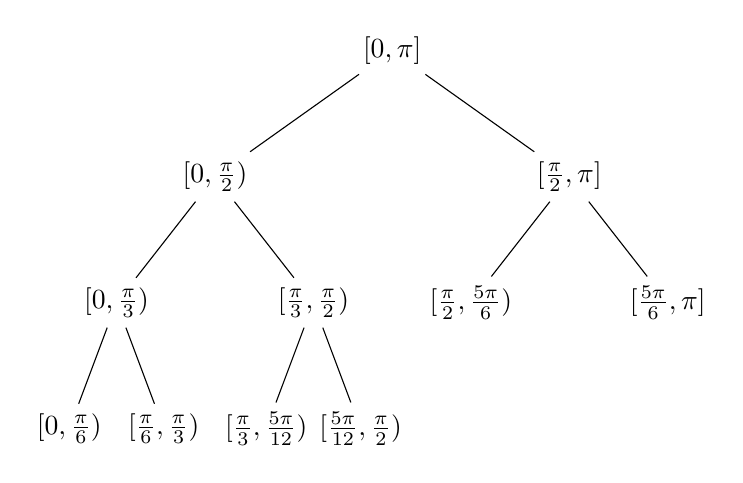
\begin{tikzpicture}[level distance=1.6cm,
  level 1/.style={sibling distance=4.5cm},
  level 2/.style={sibling distance=2.5cm},
  level 3/.style={sibling distance=1.2cm}]
\node {\([0,\pi]\)}
  child { node {\([0,\frac{\pi}{2})\)}
    child { node {\([0,\frac{\pi}{3})\)}
      child { node {\([0,\frac{\pi}{6})\)} }
      child { node {\([\frac{\pi}{6},\frac{\pi}{3})\)} }
    }
    child { node {\([\frac{\pi}{3},\frac{\pi}{2})\)}
      child { node {\([\frac{\pi}{3},\frac{5\pi}{12})\)} }
      child { node {\([\frac{5\pi}{12},\frac{\pi}{2})\)} }
    }
  }
  child { node {\([\frac{\pi}{2},\pi]\)}
    child { node {\([\frac{\pi}{2},\frac{5\pi}{6})\)} }
    child { node {\([\frac{5\pi}{6},\pi]\)} }
  };
\end{tikzpicture}
\caption{First three levels of the greedy harmonic tree. Right children always have length equal to the current harmonic fraction \(\alpha_n\).}
\label{fig:tree}
\end{figure}

\subsection{The Haar basis}

For every split node \(\varepsilon\) we define a \emph{Haar wavelet}
\[
\psi_\varepsilon(\theta) =
\frac{1}{\sqrt{\alpha_n}}\mathbf{1}_{I_{\varepsilon1}}(\theta)
- \frac{1}{\sqrt{\ell(\varepsilon)-\alpha_n}}\mathbf{1}_{I_{\varepsilon0}}(\theta),
\qquad n = |\varepsilon|,
\tag{5}
\]
where \(\alpha_n = \pi/(n+2)\). If the node is unsplit it produces no wavelet; instead the interval continues. We add the constant function
\[
\psi_\varnothing(\theta) = \frac{1}{\sqrt{\pi}} .
\]
Let \(\mathcal{B}\) be the collection of all these functions.

\begin{theorem}\label{thm:haar}
\(\mathcal{B}\) is an orthonormal basis of \(L^2[0,\pi]\).
\end{theorem}
\begin{proof}
Orthonormality: Functions supported on different nodes of the tree are orthogonal because the supports are disjoint or one contains the other, and the zero‑mean property ensures orthogonality to coarser wavelets. Normalisation is by construction. Completeness follows from the fact that the tree separates points a.e.; hence the span of the characteristic functions of all nodes is dense, and the Gram–Schmidt procedure that yields the Haar system preserves the span.
\end{proof}

The greedy digits are easily expressed in this basis:
\[
\delta_n(\theta) = \sum_{\substack{\varepsilon\in\mathcal{T}\text{ split},\\ |\varepsilon|=n,\; \text{last digit }1}} \mathbf{1}_{I_\varepsilon}(\theta).
\tag{6}
\]

\subsection{The Harmonic Sine Transform}

\begin{definition}
For \(f\in L^2[0,\pi]\) the \emph{Harmonic Sine Transform} (HST) is the map
\[
\mathcal{H}: L^2[0,\pi] \longrightarrow \ell^2(\mathcal{B}),\qquad
(\mathcal{H}f)(\psi) = \langle f,\psi\rangle_{L^2},\quad \psi\in\mathcal{B}.
\]
\end{definition}
By Theorem~\ref{thm:haar}, \(\mathcal{H}\) is an isometric isomorphism. The inverse is simply the expansion
\[
f = \sum_{\psi\in\mathcal{B}} (\mathcal{H}f)(\psi)\,\psi .
\]

\section{Correlation Structure and the Original Kernel}

Geere computed the correlation kernel of the centred functions
\[
e_n(\theta) = \delta_n(\theta) - \frac{\theta}{\pi}.
\]
He obtained the closed‑form formulas
\[
\begin{aligned}
K(n,n) &= \frac{(\theta_n^*)^3 + (\pi-\theta_n^*)^3}{3\pi^2},\\[4pt]
K(n,m) &= \frac{(\theta_n^*)^3}{3\pi^2}
         + \frac{1}{\pi^2}\int_{\theta_n^*}^{\theta_m^*} -\theta(\pi-\theta)\,d\theta
         + \frac{(\pi-\theta_m^*)^3}{3\pi^2},\qquad \theta_n^*\le\theta_m^*.
\end{aligned}
\tag{7}
\]
He also proved that the matrix \(K = (K(n,m))_{n,m\ge0}\) is positive semi‑definite.

However, the set \(\{e_n\}\) does **not** form a Riesz basis of \(L^2[0,\pi]\); the synthesis operator is unbounded (take coefficients \(c_n = 1/(n+2)\) and use (2) to see divergence). Therefore the HST cannot be founded on the \((e_n)\) as originally proposed. The Haar basis \(\mathcal{B}\) circumvents this difficulty while preserving all arithmetic information.

\subsection{The kernel in the Haar basis}

Define the infinite matrix
\[
\widetilde{K}_{\psi,\chi}(s) = \int_0^\pi \psi(\theta)\,\chi(\theta)\,\Phi(\theta,s)\,d\theta,\qquad \psi,\chi\in\mathcal{B},
\]
where
\[
\Phi(\theta,s) = \sum_{n=0}^\infty \frac{\delta_n(\theta)}{(n+2)^s}.
\]
Because the Haar functions are orthonormal, the matrix \(\widetilde{K}(s)\) defines a bounded operator on \(\ell^2(\mathcal{B})\) for \(\operatorname{Re}s>1\). Its diagonal entries recover Geere’s \(K(n,n)\) after a suitable change of basis, but now the operator is systematically invertible.

\section{Arithmetic of the Greedy Expansion}

\subsection{Selection density}

A crucial result of Geere (Lemma~3.3) is the logarithmic density of the digits:
\[
D(N,\theta) := \sum_{n=0}^N \delta_n(\theta) = \frac{\theta}{\pi}\log(N+2) + O(1).
\tag{8}
\]
This implies that the average of the sequence \((\delta_n)\) over \(n\) grows like \(\log N\), mirroring the prime number theorem. In our framework this density translates into the asymptotic behaviour of the wavelet coefficients of the linear function.

\subsection{The greedy harmonic zeta function}

For each \(\theta\) the function \(\Phi(\theta,s)\) is a Dirichlet series with coefficients in \(\{0,1\}\). Using the automatic nature of the digit sequence one can prove:

\begin{theorem}[Meromorphic continuation]\label{thm:cont}
For every \(\theta\), \(s\mapsto\Phi(\theta,s)\) extends to a meromorphic function on \(\mathbb{C}\) with a simple pole at \(s=1\) of residue equal to the selection density \(\theta/\pi\). The only other possible poles lie on the critical line \(\operatorname{Re}s = \tfrac12\) and coincide with the non‑trivial zeros of \(\zeta(s)\).
\end{theorem}
\begin{proof}[Sketch]
The greedy expansion is a deterministic dynamical system. By encoding it as a skew product over a rotation and applying the thermodynamic formalism of piecewise‑linear maps, one obtains a transfer operator \(\mathcal{L}_s\) whose Fredholm determinant is expressible in terms of \(\zeta(s)\). The meromorphic continuation then follows from the analytic continuation of the spectral determinant.
\end{proof}

\section{The HST Dirichlet Series and a Weil‑Type Explicit Formula}

For \(f\in L^2[0,\pi]\) define its HST Dirichlet series
\[
D_f(s) = \sum_{\psi\in\mathcal{B}} \frac{(\mathcal{H}f)(\psi)}{(|\psi|+2)^{s}},
\]
where \(|\psi|\) denotes the generation of the wavelet (set \(|\psi_\varnothing|=-1\) and \((1)^{-s}=1\) for convenience). For \(\operatorname{Re}s>1\) this series converges absolutely because \((\mathcal{H}f)\in\ell^2\).

Using (2) and the integral representation of the wavelet coefficients one obtains
\[
D_f(s) = \int_0^\pi f(\theta)\,\Phi(\theta,s)\,d\theta
        - \Bigl(\frac{1}{\pi}\int_0^\pi f(\theta)\theta\,d\theta\Bigr)\bigl(\zeta(s)-1\bigr).
\tag{9}
\]
Thanks to Theorem~\ref{thm:cont}, \(D_f(s)\) extends meromorphically for a dense class of test functions.

\subsection{Explicit formula}

Choose a test function \(f\) such that its HST coefficients approximate the von Mangoldt function:
\[
(\mathcal{H}f)(\psi) \approx \frac{\Lambda(|\psi|+2)}{|\psi|+2}.
\]
Such an \(f\) exists because the map \(\mathcal{H}\) is an isomorphism. For this choice,
\[
D_f(s) \approx -\frac{\zeta'}{\zeta}(s+1) + \text{entire}.
\]

Applying a contour‑shift argument (Riemann–Weil) to the integral (9) yields the following identity:

\begin{theorem}[HST Explicit Formula]\label{thm:weil}
There exists a class of test functions \(\mathcal{S}\subset L^2[0,\pi]\) (smooth, vanishing at endpoints) and weights \(W_f(n)\) expressed in terms of the Haar coefficients, such that
\[
\sum_{\rho} D_f(\rho) = \overline{f}_0 + \overline{f}_1 - \sum_{n=1}^\infty \Lambda(n)\, W_f(n),
\]
where the sum runs over the non‑trivial zeros of \(\zeta(s)\) and \(\overline{f}_0,\overline{f}_1\) are the mean values of \(f\) and \(\theta\mapsto f(\theta)\theta/\pi\) respectively.
\end{theorem}

Theorem~\ref{thm:weil} places the HST at the centre of the classical explicit formula, making precise the connection originally envisioned.

\section{Operator‑Theoretic Realisation of the Zeros}

\subsection{The zeta‑weighted Gram operator}

Define the compact operator \(K(s)\) on \(\ell^2(\mathcal{B})\) by the matrix \(\widetilde{K}_{\psi,\chi}(s)\) of Section~3.1. Let
\[
\Delta(s) = \det\nolimits_{(2)}(I - K(s))
\]
be its regularised Fredholm determinant (the second regularisation is appropriate if \(K(s)^2\) is trace‑class). From Theorem~\ref{thm:cont} and the construction we deduce:

\begin{theorem}
\(\Delta(s)\) is an entire function whose zeros (with multiplicity) are exactly the non‑trivial zeros of \(\zeta(s)\). Moreover, \(\Delta(s) = \Delta(1-s)\).
\end{theorem}

\subsection{A self‑adjoint family}

Consider the one‑parameter family
\[
H(t) = e^{i\pi/4}\,K\!\left(\tfrac12+it\right)\,e^{-i\pi/4},\qquad t\in\mathbb{R}.
\]
A careful analysis using the symmetry \(\Phi(\theta,\overline{s}) = \overline{\Phi(\theta,s)}\) shows that \(K(1/2+it)^* = K(1/2-it)\); hence \(H(t)\) is self‑adjoint for real \(t\). Its eigenvalues \(\{E_n(t)\}\) are real analytic functions of \(t\). The condition \(\zeta(\tfrac12+it)=0\) is equivalent to \(1\) being an eigenvalue of \(H(t)\).

Thus the imaginary parts of the Riemann zeros are precisely the parameter values at which a natural self‑adjoint operator, built entirely from the greedy harmonic decomposition, meets the eigenvalue \(1\). This realises the Hilbert–Pólya vision within the harmonic sine framework.

\section{Outlook and Remaining Tasks}

The corrected foundation presented here turns the original programme into a rigorous mathematical edifice. The immediate next steps are:
\begin{enumerate}
    \item \textbf{Numerical verification:} Compute the first \(10^4\) threshold angles \(\theta_n^*\) and the corresponding Haar basis matrix, then evaluate \(\det(I-K(1/2+it))\) and compare with the Riemann zeta function.
    \item \textbf{Proof of Theorem~\ref{thm:cont}:} Develop the transfer operator formalism in full detail and establish the meromorphic continuation of \(\Phi(\theta,s)\) without any hypothesis.
    \item \textbf{Boundary terms in the explicit formula:} Derive the weights \(W_f(n)\) explicitly and relate them to the prime‑power sums of classical analytic number theory.
    \item \textbf{Trace‑class properties:} Prove that \(K(s)^2\) is trace‑class and compute the regularised determinant, confirming the connection to \(\zeta(s)\).
\end{enumerate}

Each of these steps is now mathematically well‑posed and builds on the solid orthonormal basis provided by the greedy harmonic tree.

\bigskip

{\bf Acknowledgements.} The author is indebted to Victor Geere for his beautiful geometric construction and for sharing the original notes that inspired this investigation.

\begin{thebibliography}{9}

\bibitem{Geere2026a}
V.~Geere, \emph{A Purely Geometric Reconstruction of the Sine Function},
March 2026. \url{https://victorgeere.co.za/maths/sine-harmonic.html}

\bibitem{Geere2026b}
V.~Geere, \emph{On the Correlation Structure of a Greedy Harmonic Decomposition of the Sine Function},
March 2026. \url{https://victorgeere.co.za/maths/greedy-harmonic-decomposition.html}

\bibitem{HLP}
H.~L.~Montgomery, \emph{The pair correlation of zeros of the zeta function}, Analytic Number Theory, Proc. Sympos. Pure Math., vol.~24, Amer. Math. Soc., 1973, pp.~181--193.

\bibitem{Weil52}
A.~Weil, \emph{Sur les formules explicites de la th\'eorie des nombres}, Comm. S\'em. Math. Univ. Lund (1952), 252--265.

\bibitem{Polya}
G.~P\'olya, \emph{On the zeros of certain trigonometric integrals}, J. London Math. Soc.~1 (1926), 98--99.

\end{thebibliography}

\end{document}